\section{Live demo}
    \begin{frame}{Sterownik silnika}{TinyUSB (RNDIS/ECM/NCM + DHCP) + lwIP}
        \begin{itemize}
            \item STM32H5
            \item warstwa aplikacji: streamy UDP + telnet,
            \item połączenie plug \& play
        \end{itemize}
    \end{frame}

    \begin{frame}{Wizualizacja danych}{VCOM + lwIP (PPP)}
        \begin{itemize}
            \item STM32U0
            \item warstwa aplikacji: serwer HTTP + websocket
            \item łatwa integracja UI z urządzeniem
            \item lwIP nie ma wsparcia dla websocketów \\ (sam pisałem, może znajdą się na to patche)
            \item tutaj prawdopodobnie lepiej spisze się Mongoose
        \end{itemize}
        \begin{figure}[h]
            \centering
            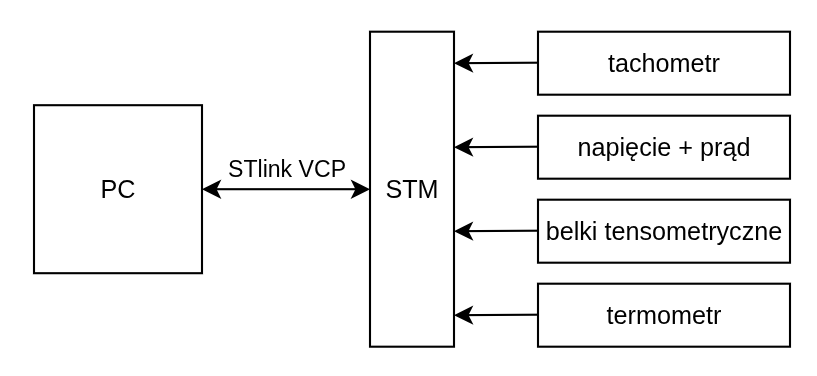
\includegraphics[width=0.75\textwidth]{images/demo2.png}
        \end{figure}
    \end{frame}

    \begin{frame}{Zadajnik PWM}{uIP (SLIP)}
        \begin{itemize}
            \item ATmega32A (2kB RAM, 32kB FLASH)
            \item za mało RAMu na lwIP, więc użyłem uIP (2003)
            \item za mało RAMu na PPP, więc użyłem SLIP
            \item warstwa aplikacji: telnet
            \item nie ma sensu ale udowadnia że się da i działa
            \item \textbf{jeśli to działa, to na innych zabytkach pewnie też}
        \end{itemize}
        \begin{figure}[h]
            \centering
            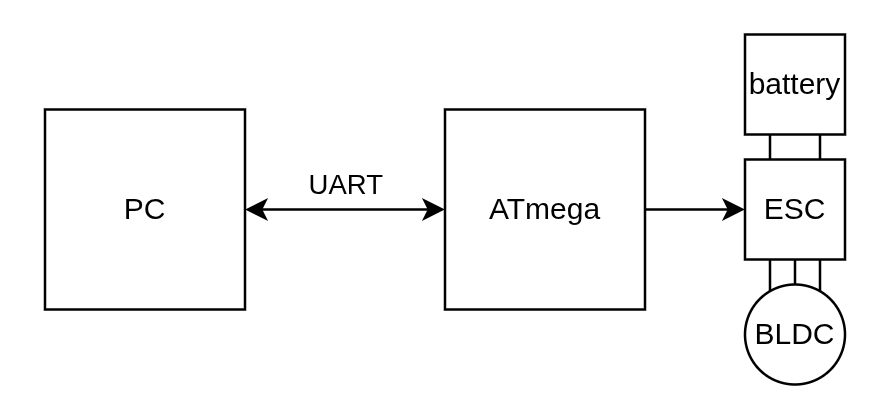
\includegraphics[width=0.6\textwidth]{images/demo3.png}
        \end{figure}
    \end{frame}

    \begin{frame}{Bieda router}{lwIP (PPP + ip forwarding)}
        \begin{itemize}
            \item STM32F4
            \item interfejsy PPP (2x UART + 1x SPI)
            \item włączona opcja "IP forwarding"
            \item umożliwia komunikację PC-STM
            \item umożlwiia komunikację STM-RPI
            \item \textbf{umożliwia komunikację PC-RPI}
            \item lwIP wymaga uwagi (patche)
        \end{itemize}
        \begin{figure}[h]
            \centering
            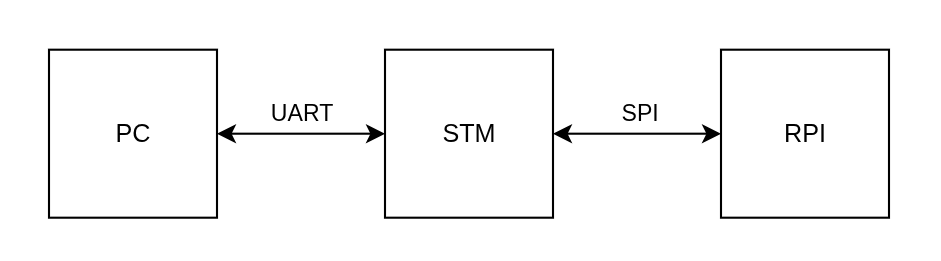
\includegraphics[width=0.75\textwidth]{images/demo4.png}
        \end{figure}
    \end{frame}

    \begin{frame}{Bieda router dla UAV}{lwIP (PPP + ip forwarding)}
        \begin{itemize}
            \item PPP działa dobrze również \textbf{bezprzewodowo}
            \item rodzaj radia nie ma znaczenia, byle dwukierunkowe (duplexowe)
            \item przepustowość UARTa nie jest górnym ograniczeniem
            \item przepustowość radia jest górnym ograniczneniem
        \end{itemize}
        \begin{figure}[h]
            \centering
            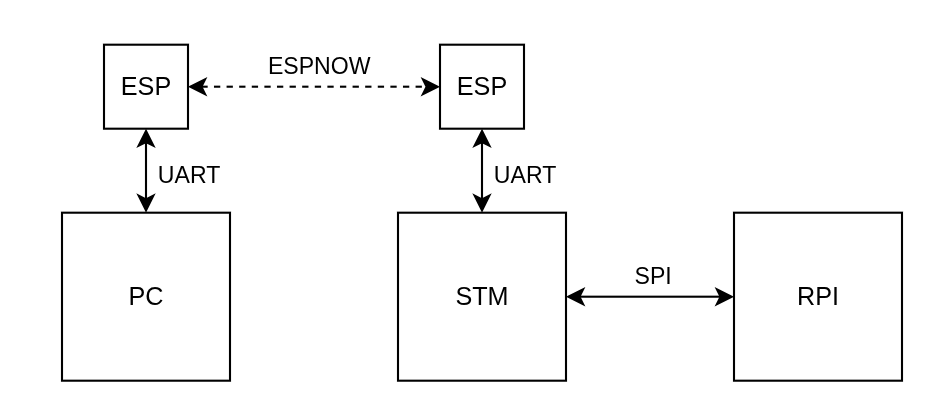
\includegraphics[width=0.75\textwidth]{images/demo4w.png}
        \end{figure}
    \end{frame}
